\documentclass[nooutcomes]{ximera}

\graphicspath{
  {./}
  {1-1QuantitativeReasoning/}
  {1-2RelationsAndGraphs/}
  {1-3ChangingInTandem/}
  {2-1LinearEquations/}
  {2-2LinearModeling/}
  {2-3ExponentialModeling/}
  {3-1WhatIsAFunction/}
  {3-2FunctionProperties/}
  {3-3AverageRatesOfChange/}
  {4-1BuildingNewFunctions/}
  {4-2Polynomials/}
  {5-1RationalFunctions/}
   {5-2ExponentialFunctions/}
  {6-1Domain/}
  {6-2Range/}
  {6-3CompositionOfFunctions/}
  {6-4FunctionTransformations/}
  {7-1ZerosOfFunctions/}
  {7-XZerosOfPolynomials/}
  {7-2ZerosOfFamousFunctions/}
  {8-1SystemsOfEquations/}
  {6-5FunctionTransformationsProject/}
  {1-1QuantitativeReasoning/exercises/}
  {1-2RelationsAndGraphs/exercises/}
  {../1-3ChangingInTandem/exercises/}
  {../2-1LinearEquations/exercises/}
  {../2-2LinearModeling/exercises/}
  {../2-3ExponentialModeling/exercises/}
  {../3-1WhatIsAFunction/exercises/}
  {../3-2FunctionProperties/exercises/}
  {../3-3AverageRatesOfChange/exercises/}
  {../5-2ExponentialFunctions/exercises/}
  {../4-1BuildingNewFunctions/exercises/}
  {../4-2Polynomials/exercises/}
  {../5-1RationalFunctions/exercises/}
  {../6-1Domain/exercises/}
  {../6-2Range/exercises/}
  {../6-3CompositionOfFunctions/exercises/}
  {../7-1ZerosOfFunctions/exercises/}
  {../7-XZerosOfPolynomials/exercises/}
  {../7-2ZerosOfFamousFunctions/exercises/}
  {../6-4FunctionTransformations/exercises/}
  {../8-1SystemsOfEquations/exercises/}
  {../6-3FunctionTransformationsProject/exercises/}
}

\DeclareGraphicsExtensions{.pdf,.png,.jpg,.eps}

\newcommand{\mooculus}{\textsf{\textbf{MOOC}\textnormal{\textsf{ULUS}}}}

\usepackage[makeroom]{cancel} %% for strike outs

\ifxake
\else
\usepackage[most]{tcolorbox}
\fi


%\typeout{************************************************}
%\typeout{New Environments}
%\typeout{************************************************}

%% to fix for web can be removed when deployed offically with ximera2
\let\image\relax\let\endimage\relax
\NewEnviron{image}{% 
  \begin{center}\BODY\end{center}% center
}



\NewEnviron{folder}{
      \addcontentsline{toc}{section}{\textbf{\BODY}}
}

\ifxake
\let\summary\relax
\let\endsummary\relax
\newtheorem*{summary}{Summary}
\newtheorem*{callout}{Callout}
\newtheorem*{overview}{Overview}
\newtheorem*{objectives}{Objectives}
\newtheorem*{motivatingQuestions}{Motivating Questions}
\newtheorem*{MM}{Metacognitive Moment}
      
%% NEEDED FOR XIMERA 2
%\ximerizedEnvironment{summary}
%\ximerizedEnvironment{callout}
%\ximerizedEnvironment{overview} 
%\ximerizedEnvironment{objectives}
%\ximerizedEnvironment{motivatingQuestions}
%\ximerizedEnvironment{MM}
\else
%% CALLOUT
\NewEnviron{callout}{
  \begin{tcolorbox}[colback=blue!5, breakable,pad at break*=1mm]
      \BODY
  \end{tcolorbox}
}
%% MOTIVATING QUESTIONS
\NewEnviron{motivatingQuestions}{
  \begin{tcolorbox}[ breakable,pad at break*=1mm]
    \textbf{\Large Motivating Questions}\hfill
    %\begin{itemize}[label=\textbullet]
      \BODY
    %\end{itemize}
  \end{tcolorbox}
}
%% OBJECTIVES
\NewEnviron{objectives}{  
    \vspace{.5in}
      %\begin{tcolorbox}[colback=orange!5, breakable,pad at break*=1mm]
    \textbf{\Large Learning Objectives}
    \begin{itemize}[label=\textbullet]
      \BODY
    \end{itemize}
    %\end{tcolorbox}
}
%% DEFINITION
\let\definition\relax
\let\enddefinition\relax
\NewEnviron{definition}{
  \begin{tcolorbox}[ breakable,pad at break*=1mm]
    \noindent\textbf{Definition}~
      \BODY
  \end{tcolorbox}
}
%% OVERVIEW
\let\overview\relax
\let\overview\relax
\NewEnviron{overview}{
  \begin{tcolorbox}[ breakable,pad at break*=1mm]
    \textbf{\Large Overview}
    %\begin{itemize}[label=\textbullet] %% breaks Xake
      \BODY
    %\end{itemize}
  \end{tcolorbox}
}
%% SUMMARY
\let\summary\relax
\let\endsummary\relax
\NewEnviron{summary}{
  \begin{tcolorbox}[ breakable,pad at break*=1mm]
    \textbf{\Large Summary}
    %\begin{itemize}[label=\textbullet] %% breaks Xake
      \BODY
    %\end{itemize}
  \end{tcolorbox}
}
%% REMARK
\let\remark\relax
\let\endremark\relax
\NewEnviron{remark}{
  \begin{tcolorbox}[colback=green!5, breakable,pad at break*=1mm]
    \noindent\textbf{Remark}~
      \BODY
  \end{tcolorbox}
}
%% EXPLANATION
\let\explanation\relax
\let\endexplanation\relax
\NewEnviron{explanation}{
    \normalfont
    \noindent\textbf{Explanation}~
      \BODY
}
%% EXPLORATION
\let\exploration\relax
\let\endexploration\relax
\NewEnviron{exploration}{
  \begin{tcolorbox}[colback=yellow!10, breakable,pad at break*=1mm]
    \noindent\textbf{Exploration}~
      \BODY
  \end{tcolorbox}
}
%% METACOGNITIVE MOMENTS
\let\MM\relax
\let\endMM\relax
\NewEnviron{MM}{
  \begin{tcolorbox}[colback=pink!15, breakable,pad at break*=1mm]
    \noindent\textbf{Metacognitive Moment}~
      \BODY
  \end{tcolorbox}
}


\fi





%Notes on what envirnoment to use:  Example with Explanation in text; if they are supposed to answer- Problem; no answer - Exploration


%\typeout{************************************************}
%% Header and footers
%\typeout{************************************************}

\newcommand{\licenseAcknowledgement}{Licensed under Creative Commons 4.0}
\newcommand{\licenseAPC}{\renewcommand{\licenseAcknowledgement}{\textbf{Acknowledgements:} Active Prelude to Calculus (https://activecalculus.org/prelude) }}
\newcommand{\licenseSZ}{\renewcommand{\licenseAcknowledgement}{\textbf{Acknowledgements:} Stitz Zeager Open Source Mathematics (https://www.stitz-zeager.com/) }}
\newcommand{\licenseAPCSZ}{\renewcommand{\licenseAcknowledgement}{\textbf{Acknowledgements:} Active Prelude to Calculus (https://activecalculus.org/prelude) and Stitz Zeager Open Source Mathematics (https://www.stitz-zeager.com/) }}
\newcommand{\licenseORCCA}{\renewcommand{\licenseAcknowledgement}{\textbf{Acknowledgements:}Original source material, products with readable and accessible
math content, and other information freely available at pcc.edu/orcca.}}
\newcommand{\licenseY}{\renewcommand{\licenseAcknowledgement}{\textbf{Acknowledgements:} Yoshiwara Books (https://yoshiwarabooks.org/)}}
\newcommand{\licenseOS}{\renewcommand{\licenseAcknowledgement}{\textbf{Acknowledgements:} OpenStax College Algebra (https://openstax.org/details/books/college-algebra)}}
\newcommand{\licenseAPCSZCSCC}{\renewcommand{\licenseAcknowledgement}{\textbf{Acknowledgements:} Active Prelude to Calculus (https://activecalculus.org/prelude), Stitz Zeager Open Source Mathematics (https://www.stitz-zeager.com/), CSCC PreCalculus and Calculus texts (https://ximera.osu.edu/csccmathematics)}}

\ifxake\else %% do nothing on the website
\usepackage{fancyhdr}
\pagestyle{fancy}
\fancyhf{}
\fancyhead[R]{\sectionmark}
\fancyfoot[L]{\thepage}
\fancyfoot[C]{\licenseAcknowledgement}
\renewcommand{\headrulewidth}{0pt}
\renewcommand{\footrulewidth}{0pt}
\fi

%%%%%%%%%%%%%%%%



%\typeout{************************************************}
%\typeout{Table of Contents}
%\typeout{************************************************}


%% Edit this to change the font style
\newcommand{\sectionHeadStyle}{\sffamily\bfseries}


\makeatletter

%% part uses arabic numerals
\renewcommand*\thepart{\arabic{part}}


\ifxake\else
\renewcommand\chapterstyle{%
  \def\maketitle{%
    \addtocounter{titlenumber}{1}%
    \pagestyle{fancy}
    \phantomsection
    \addcontentsline{toc}{section}{\textbf{\thepart.\thetitlenumber\hspace{1em}\@title}}%
                    {\flushleft\small\sectionHeadStyle\@pretitle\par\vspace{-1.5em}}%
                    {\flushleft\LARGE\sectionHeadStyle\thepart.\thetitlenumber\hspace{1em}\@title \par }%
                    {\setcounter{problem}{0}\setcounter{sectiontitlenumber}{0}}%
                    \par}}





\renewcommand\sectionstyle{%
  \def\maketitle{%
    \addtocounter{sectiontitlenumber}{1}
    \pagestyle{fancy}
    \phantomsection
    \addcontentsline{toc}{subsection}{\thepart.\thetitlenumber.\thesectiontitlenumber\hspace{1em}\@title}%
    {\flushleft\small\sectionHeadStyle\@pretitle\par\vspace{-1.5em}}%
    {\flushleft\Large\sectionHeadStyle\thepart.\thetitlenumber.\thesectiontitlenumber\hspace{1em}\@title \par}%
    %{\setcounter{subsectiontitlenumber}{0}}%
    \par}}



\renewcommand\section{\@startsection{paragraph}{10}{\z@}%
                                     {-3.25ex\@plus -1ex \@minus -.2ex}%
                                     {1.5ex \@plus .2ex}%
                                     {\normalfont\large\sectionHeadStyle}}
\renewcommand\subsection{\@startsection{subparagraph}{10}{\z@}%
                                    {3.25ex \@plus1ex \@minus.2ex}%
                                    {-1em}%
                                    {\normalfont\normalsize\sectionHeadStyle}}

\fi

%% redefine Part
\renewcommand\part{%
   {\setcounter{titlenumber}{0}}
  \if@openright
    \cleardoublepage
  \else
    \clearpage
  \fi
  \thispagestyle{plain}%
  \if@twocolumn
    \onecolumn
    \@tempswatrue
  \else
    \@tempswafalse
  \fi
  \null\vfil
  \secdef\@part\@spart}

\def\@part[#1]#2{%
    \ifnum \c@secnumdepth >-2\relax
      \refstepcounter{part}%
      \addcontentsline{toc}{part}{\thepart\hspace{1em}#1}%
    \else
      \addcontentsline{toc}{part}{#1}%
    \fi
    \markboth{}{}%
    {\centering
     \interlinepenalty \@M
     \normalfont
     \ifnum \c@secnumdepth >-2\relax
       \huge\sffamily\bfseries \partname\nobreakspace\thepart
       \par
       \vskip 20\p@
     \fi
     \Huge \bfseries #2\par}%
    \@endpart}
\def\@spart#1{%
    {\centering
     \interlinepenalty \@M
     \normalfont
     \Huge \bfseries #1\par}%
    \@endpart}
\def\@endpart{\vfil\newpage
              \if@twoside
               \if@openright
                \null
                \thispagestyle{empty}%
                \newpage
               \fi
              \fi
              \if@tempswa
                \twocolumn
                \fi}



\makeatother





%\typeout{************************************************}
%\typeout{Stuff from Ximera}
%\typeout{************************************************}



\usepackage{array}  %% This is for typesetting long division
\setlength{\extrarowheight}{+.1cm}
\newdimen\digitwidth
\settowidth\digitwidth{9}
\def\divrule#1#2{
\noalign{\moveright#1\digitwidth
\vbox{\hrule width#2\digitwidth}}}





\newcommand{\RR}{\mathbb R}
\newcommand{\R}{\mathbb R}
\newcommand{\N}{\mathbb N}
\newcommand{\Z}{\mathbb Z}

\newcommand{\sagemath}{\textsf{SageMath}}


\def\d{\,d}
%\renewcommand{\d}{\mathop{}\!d}
\newcommand{\dd}[2][]{\frac{\d #1}{\d #2}}
\newcommand{\pp}[2][]{\frac{\partial #1}{\partial #2}}
\renewcommand{\l}{\ell}
\newcommand{\ddx}{\frac{d}{\d x}}



%\newcommand{\unit}{\,\mathrm}
\newcommand{\unit}{\mathop{}\!\mathrm}
\newcommand{\eval}[1]{\bigg[ #1 \bigg]}
\newcommand{\seq}[1]{\left( #1 \right)}
\renewcommand{\epsilon}{\varepsilon}
\renewcommand{\phi}{\varphi}


\renewcommand{\iff}{\Leftrightarrow}

\DeclareMathOperator{\arccot}{arccot}
\DeclareMathOperator{\arcsec}{arcsec}
\DeclareMathOperator{\arccsc}{arccsc}
\DeclareMathOperator{\sign}{sign}


%\DeclareMathOperator{\divergence}{divergence}
%\DeclareMathOperator{\curl}[1]{\grad\cross #1}
\newcommand{\lto}{\mathop{\longrightarrow\,}\limits}

\renewcommand{\bar}{\overline}

\colorlet{textColor}{black}
\colorlet{background}{white}
\colorlet{penColor}{blue!50!black} % Color of a curve in a plot
\colorlet{penColor2}{red!50!black}% Color of a curve in a plot
\colorlet{penColor3}{red!50!blue} % Color of a curve in a plot
\colorlet{penColor4}{green!50!black} % Color of a curve in a plot
\colorlet{penColor5}{orange!80!black} % Color of a curve in a plot
\colorlet{penColor6}{yellow!70!black} % Color of a curve in a plot
\colorlet{fill1}{penColor!20} % Color of fill in a plot
\colorlet{fill2}{penColor2!20} % Color of fill in a plot
\colorlet{fillp}{fill1} % Color of positive area
\colorlet{filln}{penColor2!20} % Color of negative area
\colorlet{fill3}{penColor3!20} % Fill
\colorlet{fill4}{penColor4!20} % Fill
\colorlet{fill5}{penColor5!20} % Fill
\colorlet{gridColor}{gray!50} % Color of grid in a plot

\newcommand{\surfaceColor}{violet}
\newcommand{\surfaceColorTwo}{redyellow}
\newcommand{\sliceColor}{greenyellow}




\pgfmathdeclarefunction{gauss}{2}{% gives gaussian
  \pgfmathparse{1/(#2*sqrt(2*pi))*exp(-((x-#1)^2)/(2*#2^2))}%
}





%\typeout{************************************************}
%\typeout{ORCCA Preamble.Tex}
%\typeout{************************************************}


%% \usepackage{geometry}
%% \geometry{letterpaper,total={408pt,9.0in}}
%% Custom Page Layout Adjustments (use latex.geometry)
%% \usepackage{amsmath,amssymb}
%% \usepackage{pgfplots}
\usepackage{pifont}                                         %needed for symbols, s.a. airplane symbol
\usetikzlibrary{positioning,fit,backgrounds}                %needed for nested diagrams
\usetikzlibrary{calc,trees,positioning,arrows,fit,shapes}   %needed for set diagrams
\usetikzlibrary{decorations.text}                           %needed for text following a curve
\usetikzlibrary{arrows,arrows.meta}                         %needed for open/closed intervals
\usetikzlibrary{positioning,3d,shapes.geometric}            %needed for 3d number sets tower

%% NEEDED FOR XIMERA 1
%\usetkzobj{all}       %NO LONGER VALID
%%%%%%%%%%%%%%

\usepackage{tikz-3dplot}
\usepackage{tkz-euclide}                     %needed for triangle diagrams
\usepgfplotslibrary{fillbetween}                            %shade regions of a plot
\usetikzlibrary{shadows}                                    %function diagrams
\usetikzlibrary{positioning}                                %function diagrams
\usetikzlibrary{shapes}                                     %function diagrams
%%% global colors from https://www.pcc.edu/web-services/style-guide/basics/color/ %%%
\definecolor{ruby}{HTML}{9E0C0F}
\definecolor{turquoise}{HTML}{008099}
\definecolor{emerald}{HTML}{1c8464}
\definecolor{amber}{HTML}{c7502a}
\definecolor{amethyst}{HTML}{70485b}
\definecolor{sapphire}{HTML}{263c53}
\colorlet{firstcolor}{sapphire}
\colorlet{secondcolor}{turquoise}
\colorlet{thirdcolor}{emerald}
\colorlet{fourthcolor}{amber}
\colorlet{fifthcolor}{amethyst}
\colorlet{sixthcolor}{ruby}
\colorlet{highlightcolor}{green!50!black}
\colorlet{graphbackground}{white}
\colorlet{wood}{brown!60!white}
%%% curve, dot, and graph custom styles %%%
\pgfplotsset{firstcurve/.style      = {color=firstcolor,  mark=none, line width=1pt, {Kite}-{Kite}, solid}}
\pgfplotsset{secondcurve/.style     = {color=secondcolor, mark=none, line width=1pt, {Kite}-{Kite}, solid}}
\pgfplotsset{thirdcurve/.style      = {color=thirdcolor,  mark=none, line width=1pt, {Kite}-{Kite}, solid}}
\pgfplotsset{fourthcurve/.style     = {color=fourthcolor, mark=none, line width=1pt, {Kite}-{Kite}, solid}}
\pgfplotsset{fifthcurve/.style      = {color=fifthcolor,  mark=none, line width=1pt, {Kite}-{Kite}, solid}}
\pgfplotsset{highlightcurve/.style  = {color=highlightcolor,  mark=none, line width=5pt, -, opacity=0.3}}   % thick, opaque curve for highlighting
\pgfplotsset{asymptote/.style       = {color=gray, mark=none, line width=1pt, <->, dashed}}
\pgfplotsset{symmetryaxis/.style    = {color=gray, mark=none, line width=1pt, <->, dashed}}
\pgfplotsset{guideline/.style       = {color=gray, mark=none, line width=1pt, -}}
\tikzset{guideline/.style           = {color=gray, mark=none, line width=1pt, -}}
\pgfplotsset{altitude/.style        = {dashed, color=gray, thick, mark=none, -}}
\tikzset{altitude/.style            = {dashed, color=gray, thick, mark=none, -}}
\pgfplotsset{radius/.style          = {dashed, thick, mark=none, -}}
\tikzset{radius/.style              = {dashed, thick, mark=none, -}}
\pgfplotsset{rightangle/.style      = {color=gray, mark=none, -}}
\tikzset{rightangle/.style          = {color=gray, mark=none, -}}
\pgfplotsset{closedboundary/.style  = {color=black, mark=none, line width=1pt, {Kite}-{Kite},solid}}
\tikzset{closedboundary/.style      = {color=black, mark=none, line width=1pt, {Kite}-{Kite},solid}}
\pgfplotsset{openboundary/.style    = {color=black, mark=none, line width=1pt, {Kite}-{Kite},dashed}}
\tikzset{openboundary/.style        = {color=black, mark=none, line width=1pt, {Kite}-{Kite},dashed}}
\tikzset{verticallinetest/.style    = {color=gray, mark=none, line width=1pt, <->,dashed}}
\pgfplotsset{soliddot/.style        = {color=firstcolor,  mark=*, only marks}}
\pgfplotsset{hollowdot/.style       = {color=firstcolor,  mark=*, only marks, fill=graphbackground}}
\pgfplotsset{blankgraph/.style      = {xmin=-10, xmax=10,
                                        ymin=-10, ymax=10,
                                        axis line style={-, draw opacity=0 },
                                        axis lines=box,
                                        major tick length=0mm,
                                        xtick={-10,-9,...,10},
                                        ytick={-10,-9,...,10},
                                        grid=major,
                                        grid style={solid,gray!20},
                                        xticklabels={,,},
                                        yticklabels={,,},
                                        minor xtick=,
                                        minor ytick=,
                                        xlabel={},ylabel={},
                                        width=0.75\textwidth,
                                      }
            }
\pgfplotsset{numberline/.style      = {xmin=-10,xmax=10,
                                        minor xtick={-11,-10,...,11},
                                        xtick={-10,-5,...,10},
                                        every tick/.append style={thick},
                                        axis y line=none,
                                        y=15pt,
                                        axis lines=middle,
                                        enlarge x limits,
                                        grid=none,
                                        clip=false,
                                        axis background/.style={},
                                        after end axis/.code={
                                          \path (axis cs:0,0)
                                          node [anchor=north,yshift=-0.075cm] {\footnotesize 0};
                                        },
                                        every axis x label/.style={at={(current axis.right of origin)},anchor=north},
                                      }
            }
\pgfplotsset{openinterval/.style={color=firstcolor,mark=none,ultra thick,{Parenthesis}-{Parenthesis}}}
\pgfplotsset{openclosedinterval/.style={color=firstcolor,mark=none,ultra thick,{Parenthesis}-{Bracket}}}
\pgfplotsset{closedinterval/.style={color=firstcolor,mark=none,ultra thick,{Bracket}-{Bracket}}}
\pgfplotsset{closedopeninterval/.style={color=firstcolor,mark=none,ultra thick,{Bracket}-{Parenthesis}}}
\pgfplotsset{infiniteopeninterval/.style={color=firstcolor,mark=none,ultra thick,{Kite}-{Parenthesis}}}
\pgfplotsset{openinfiniteinterval/.style={color=firstcolor,mark=none,ultra thick,{Parenthesis}-{Kite}}}
\pgfplotsset{infiniteclosedinterval/.style={color=firstcolor,mark=none,ultra thick,{Kite}-{Bracket}}}
\pgfplotsset{closedinfiniteinterval/.style={color=firstcolor,mark=none,ultra thick,{Bracket}-{Kite}}}
\pgfplotsset{infiniteinterval/.style={color=firstcolor,mark=none,ultra thick,{Kite}-{Kite}}}
\pgfplotsset{interval/.style= {ultra thick, -}}
%%% cycle list of plot styles for graphs with multiple plots %%%
\pgfplotscreateplotcyclelist{pccstylelist}{%
  firstcurve\\%
  secondcurve\\%
  thirdcurve\\%
  fourthcurve\\%
  fifthcurve\\%
}
%%% default plot settings %%%
\pgfplotsset{every axis/.append style={
  axis x line=middle,    % put the x axis in the middle
  axis y line=middle,    % put the y axis in the middle
  axis line style={<->}, % arrows on the axis
  scaled ticks=false,
  tick label style={/pgf/number format/fixed},
  xlabel={$x$},          % default put x on x-axis
  ylabel={$y$},          % default put y on y-axis
  xmin = -7,xmax = 7,    % most graphs have this window
  ymin = -7,ymax = 7,    % most graphs have this window
  domain = -7:7,
  xtick = {-6,-4,...,6}, % label these ticks
  ytick = {-6,-4,...,6}, % label these ticks
  yticklabel style={inner sep=0.333ex},
  minor xtick = {-7,-6,...,7}, % include these ticks, some without label
  minor ytick = {-7,-6,...,7}, % include these ticks, some without label
  scale only axis,       % don't consider axis and tick labels for width and height calculation
  cycle list name=pccstylelist,
  tick label style={font=\footnotesize},
  legend cell align=left,
  grid = both,
  grid style = {solid,gray!20},
  axis background/.style={fill=graphbackground},
}}
\pgfplotsset{framed/.style={axis background/.style ={draw=gray}}}
%\pgfplotsset{framed/.style={axis background/.style ={draw=gray,fill=graphbackground,rounded corners=3ex}}}
%%% other tikz (not pgfplots) settings %%%
%\tikzset{axisnode/.style={font=\scriptsize,text=black}}
\tikzset{>=stealth}
%%% for nested diagram in types of numbers section %%%
\newcommand\drawnestedsets[4]{
  \def\position{#1}             % initial position
  \def\nbsets{#2}               % number of sets
  \def\listofnestedsets{#3}     % list of sets
  \def\reversedlistofcolors{#4} % reversed list of colors
  % position and draw labels of sets
  \coordinate (circle-0) at (#1);
  \coordinate (set-0) at (#1);
  \foreach \set [count=\c] in \listofnestedsets {
    \pgfmathtruncatemacro{\cminusone}{\c - 1}
    % label of current set (below previous nested set)
    \node[below=3pt of circle-\cminusone,inner sep=0]
    (set-\c) {\set};
    % current set (fit current label and previous set)
    \node[circle,inner sep=0,fit=(circle-\cminusone)(set-\c)]
    (circle-\c) {};
  }
  % draw and fill sets in reverse order
  \begin{scope}[on background layer]
    \foreach \col[count=\c] in \reversedlistofcolors {
      \pgfmathtruncatemacro{\invc}{\nbsets-\c}
      \pgfmathtruncatemacro{\invcplusone}{\invc+1}
      \node[circle,draw,fill=\col,inner sep=0,
      fit=(circle-\invc)(set-\invcplusone)] {};
    }
  \end{scope}
  }
\ifdefined\tikzset
\tikzset{ampersand replacement = \amp}
\fi
\newcommand{\abs}[1]{\left\lvert#1\right\rvert}
%\newcommand{\point}[2]{\left(#1,#2\right)}
\newcommand{\highlight}[1]{\definecolor{sapphire}{RGB}{59,90,125} {\color{sapphire}{{#1}}}}
\newcommand{\firsthighlight}[1]{\definecolor{sapphire}{RGB}{59,90,125} {\color{sapphire}{{#1}}}}
\newcommand{\secondhighlight}[1]{\definecolor{emerald}{RGB}{20,97,75} {\color{emerald}{{#1}}}}
\newcommand{\unhighlight}[1]{{\color{black}{{#1}}}}
\newcommand{\lowlight}[1]{{\color{lightgray}{#1}}}
\newcommand{\attention}[1]{\mathord{\overset{\downarrow}{#1}}}
\newcommand{\nextoperation}[1]{\mathord{\boxed{#1}}}
\newcommand{\substitute}[1]{{\color{blue}{{#1}}}}
\newcommand{\pinover}[2]{\overset{\overset{\mathrm{\ #2\ }}{|}}{\strut #1 \strut}}
\newcommand{\addright}[1]{{\color{blue}{{{}+#1}}}}
\newcommand{\addleft}[1]{{\color{blue}{{#1+{}}}}}
\newcommand{\subtractright}[1]{{\color{blue}{{{}-#1}}}}
\newcommand{\multiplyright}[2][\cdot]{{\color{blue}{{{}#1#2}}}}
\newcommand{\multiplyleft}[2][\cdot]{{\color{blue}{{#2#1{}}}}}
\newcommand{\divideunder}[2]{\frac{#1}{{\color{blue}{{#2}}}}}
\newcommand{\divideright}[1]{{\color{blue}{{{}\div#1}}}}
\newcommand{\negate}[1]{{\color{blue}{{-}}}\left(#1\right)}
\newcommand{\cancelhighlight}[1]{\definecolor{sapphire}{RGB}{59,90,125}{\color{sapphire}{{\cancel{#1}}}}}
\newcommand{\secondcancelhighlight}[1]{\definecolor{emerald}{RGB}{20,97,75}{\color{emerald}{{\bcancel{#1}}}}}
\newcommand{\thirdcancelhighlight}[1]{\definecolor{amethyst}{HTML}{70485b}{\color{amethyst}{{\xcancel{#1}}}}}
\newcommand{\lt}{<} %% Bart: WHY?
\newcommand{\gt}{>} %% Bart: WHY?
\newcommand{\amp}{&} %% Bart: WHY?


%%% These commands break Xake
%% \newcommand{\apple}{\text{🍎}}
%% \newcommand{\banana}{\text{🍌}}
%% \newcommand{\pear}{\text{🍐}}
%% \newcommand{\cat}{\text{🐱}}
%% \newcommand{\dog}{\text{🐶}}

\newcommand{\apple}{PICTURE OF APPLE}
\newcommand{\banana}{PICTURE OF BANANA}
\newcommand{\pear}{PICTURE OF PEAR}
\newcommand{\cat}{PICTURE OF CAT}
\newcommand{\dog}{PICTURE OF DOG}


%%%%% INDEX STUFF
\newcommand{\dfn}[1]{\textbf{#1}\index{#1}}
\usepackage{imakeidx}
\makeindex[intoc]
\makeatletter
\gdef\ttl@savemark{\sectionmark{}}
\makeatother












 % for drawing cube in Optimization problem
\usetikzlibrary{quotes,arrows.meta}
\tikzset{
  annotated cuboid/.pic={
    \tikzset{%
      every edge quotes/.append style={midway, auto},
      /cuboid/.cd,
      #1
    }
    \draw [every edge/.append style={pic actions, densely dashed, opacity=.5}, pic actions]
    (0,0,0) coordinate (o) -- ++(-\cubescale*\cubex,0,0) coordinate (a) -- ++(0,-\cubescale*\cubey,0) coordinate (b) edge coordinate [pos=1] (g) ++(0,0,-\cubescale*\cubez)  -- ++(\cubescale*\cubex,0,0) coordinate (c) -- cycle
    (o) -- ++(0,0,-\cubescale*\cubez) coordinate (d) -- ++(0,-\cubescale*\cubey,0) coordinate (e) edge (g) -- (c) -- cycle
    (o) -- (a) -- ++(0,0,-\cubescale*\cubez) coordinate (f) edge (g) -- (d) -- cycle;
    \path [every edge/.append style={pic actions, |-|}]
    (b) +(0,-5pt) coordinate (b1) edge ["x"'] (b1 -| c)
    (b) +(-5pt,0) coordinate (b2) edge ["y"] (b2 |- a)
    (c) +(3.5pt,-3.5pt) coordinate (c2) edge ["x"'] ([xshift=3.5pt,yshift=-3.5pt]e)
    ;
  },
  /cuboid/.search also={/tikz},
  /cuboid/.cd,
  width/.store in=\cubex,
  height/.store in=\cubey,
  depth/.store in=\cubez,
  units/.store in=\cubeunits,
  scale/.store in=\cubescale,
  width=10,
  height=10,
  depth=10,
  units=cm,
  scale=.1,
}

\author{Kenneth Berglund}
\license{Creative Commons Attribution-ShareAlike 4.0 International License}
\acknowledgement{https://activecalculus.org/, stitz-zeager}

\title{Inverse Functions}

\begin{document}
\licenseAPCSZ
\begin{abstract}
  
\end{abstract}
\maketitle


%\typeout{************************************************}
%\typeout{Motivating Questions}
%\typeout{************************************************}

\begin{motivatingQuestions}\begin{itemize}
\item What does it mean to say that a function has an inverse? 
\item How can we identify when we can find inverse functions?
\item What are the properties of an inverse function compared to the original function?
\end{itemize}\end{motivatingQuestions}


%\typeout{************************************************}
%\typeout{Introduction}
%\typeout{************************************************}

Because every function is a process that converts a collection of inputs to a corresponding collection of outputs, a natural question is: for a particular function, can we change perspective and think of the original function's outputs as the inputs for a reverse process? If we phrase this question algebraically, it is analogous to asking: given an equation that defines $y$ is a function of $x$, is it possible to find a corresponding equation where $x$ is a function of $y$?


%\typeout{************************************************}
%\typeout{Inverse functions}
%\typeout{************************************************}

\section{Inverse functions}
Let's think about the problem in a more concrete way. Consider a situation in which Jessica is running a candle company. Say she starts the day with \$15, but makes \$4 for every candle she sells. A linear function $f$ representing the amount of money in dollars she has after selling $x$ candles is given by $f(x) = 4x + 15$. To find out how much money she has after selling 20 candles, we can plug in 20 to the equation above:
$$
f(20) = 4\cdot 20 + 15 = 95.
$$

Now suppose that Jessica tells us that at the end of the day, she ended up with \$135. Would it be possible to figure out how many candles she sold? This type of ``inverse question'' is common in math. Notice that above, when we started with an amount of candles and wanted to find an amount of money, we first multiplied by 4, then added 15. Now, since we're starting with an amount of money, we need to undo the processes we did before: first we subtract 15, and then divide by 4.  We can represent this process by a function $g$, which represents the number of candles sold if Jessica has $y$ dollars:
$$
g(y) = \frac{1}{4}(y - 15).
$$

When we plug in \$135 to this function, we find that Jessica has sold
$$
g(135) = \frac{1}{4}(135 - 15) = 30
$$
candles. 

\begin{exploration}
Let $f$ be a function defined by $f(x) = 4x + 15$. Let $g$ be a function defined by $g(y) = \frac{1}{4}(y - 15)$.
\begin{enumerate}[label=\alph*.]
\item Recall that $f(20) = 95$. What is $g(95)$?
\item Recall that $g(135) = 30$. What is $f(30)$?
\end{enumerate}
\end{exploration}

After plugging in, we see that when we plug 20 into $f$, we get $f(20) = 95$, and when we plug 95 into $g$ (that is, we plug $f(20)$ into $g$), we get back 20. Similarly, when we plug in the value $g(135)$ into $f$, we get back 135. The following diagram illustrates the situation:
\begin{image}
\begin{tikzpicture}[
roundnode/.style={shape=circle,font=\fontsize{12}{12}\selectfont, draw=black, thick}
]
%Nodes
\node[roundnode]      (20)                              {20};
\node[roundnode]        (95)       [right=of 20] {95};
\node[roundnode]      (30)       [below=of 20] {30};
\node[roundnode]        (135)       [right=of 30] {135};

%Lines
\draw[->, color=penColor] (20) to [out=20,in=160]node[above]{$f$} (95) ;
\draw[->, color=penColor2] (95) to [out=200,in=340]node[below]{$g$}(20) ;
\draw[->, color=penColor] (30) to [out=20,in=160]node[above]{$f$} (135) ;
\draw[->, color=penColor2] (135) to [out=200,in=340]node[below]{$g$} (30) ;
\end{tikzpicture}
\end{image}

In the above exploration, $f$ and $g$ are examples of \emph{inverse functions}. 

\begin{definition}
Let $f$ be a function. If there exists a function $g$ such that
$$
g(f(a)) = a \text{ and } f(g(b)) = b
$$
for each $a$ and $b$, then we say that $f$ has an \index{function ! inverse}\index{inverse function}\index{inverse}\dfn{inverse function} and that the function $g$ is the \dfn{inverse} of $f$. We also say that $f$ is \index{function ! invertible}\index{invertible}\dfn{invertible}. 
\end{definition}

Note particularly what the equation $g(f(a)) = a$ says:  for any input $a$, the function $g$ will reverse the process of $f$ (which converts $a$ to $f(a)$) because $g$ converts $f(a)$ back to $a$.

When a given function $f$ has a corresponding inverse function $g$, we usually rename $g$ as $f^{-1}$, which we read aloud as ``$f$-inverse''. The equation $g(f(a)) = a$ now reads as $f^{-1}(f(a)) = a$, which we interpret as saying ``$f$-inverse converts $f(a)$ back to $a$''. We similarly write that $f(f^{-1}(b)) = b$. 

\begin{exploration}
Dolbear's function $F = D(N) = 40 + \frac{1}{4}N$ is used to model the number $N$ of snowy tree cricket chirps per minute to a corresponding Fahrenheit temperature. 
\begin{enumerate}[label=\alph*.]
\item Solve the equation $F = 40 + \frac{1}{4}N$ for $N$ in terms of $F$. Call the resulting function $N = E(F)$. 
\item Explain in words the process or effect of the function $N = E(F)$. What does it take as input? What does it generate as output?
\item Use the function $E$ that you found above to compute $j(N) = E(D(N))$. Simplify your result as much as possible. Do likewise for $k(F) = D(E(F))$. What do you notice about these two functions $j$ and $k$?
\item Consider the equations $F = 40 + \frac{1}{4}N$ and $N = 4(F - 40)$. Do these equations express different relationships between $F$ and $N$, or do they express the same relationship in two different ways? Explain. 
\end{enumerate}
\end{exploration}

When a given function has an inverse function, it allows us to express the same relationship from two different points of view.  For instance, if $y = f(t) = 2t + 1$, we can show that the function $t = g(y) = \frac{y-1}{2}$ reverses the effect of $f$ (and vice versa), and thus $g = f^{-1}$.  We observe that 
$$
y = f(t) = 2t + 1 \text{ and } t = f^{-1}(y) = \frac{y-1}{2}
$$
are equivalent forms of the same equation, and thus they say the same thing from two different perspectives.  The first version of the equation is solved for $y$ in terms of $t$, while the second equation is solved for $t$ in terms of $y$.  This important principle holds in general whenever a function has an inverse function.

If $y = f(t)$ has an inverse function, then the equations
$$
y = f(t) \text{ and } t = f^{-1}(y)
$$
say the exact same thing but from two different perspectives. 

%\typeout{************************************************}
%\typeout{When can we find inverses?}
%\typeout{************************************************}

\section{When can we find inverses?}
 It's important to note in the above definition of inverse functions that we say ``\emph{If} there exists $\ldots$''.  That is, we don't guarantee that an inverse function exists for a given function.  Thus, we might ask: how can we determine whether or not a given function has a corresponding inverse function?  As with many questions about functions, there are often three different possible ways to explore such a question:  through a table, through a graph, or through an algebraic formula.

Consider the functions $f$ and $g$ given in the following tables. 

\begin{center}
$
\begin{array}{ |c || c|  }
 \hline
 x & f(x)\\
 \hline
 0&6\\
 1&4\\
 2&3\\
 3&4\\
 4&6\\
 \hline
\end{array} 
$
\hspace{2cm}
$
\begin{array}{ |c || c|  }
 \hline
 x & g(x)\\
 \hline
 0&3\\
 1&1\\
 2&4\\
 3&2\\
 4&0\\
 \hline
\end{array} 
$
\end{center}

For any function, the question of whether or not it has an inverse comes down to whether or not the process of the function can be reliably reversed.  For functions given in table form such as $f$ and $g$, we essentially ask if it's possible to swich the input and output columns and have the new resulting table also represent a function.

The function $f$ does not have an inverse function because there are two different inputs that lead to the same output:  $f(0) = 6$ and $f(4) = 6$.  If we attempt to reverse this process, we have a situation where the input $6$ would correspond to \emph{two} potential outputs, $4$ and $6$.

However, the function $g$ does have an inverse function because when we reverse the columns in the table each input (in order, $3$, $1$, $4$, $2$, $0$) indeed corresponds to one and only one output (in order, $0$, $1$, $2$, $3$, $4$).  We can thus make observations such as $g^{-1}(4) = 2$, which is the same as saying that $g(2) = 4$, just from a different perspective.

Now, consider the functions  $p$ and $q$ represented by the following graphs.

\begin{image}
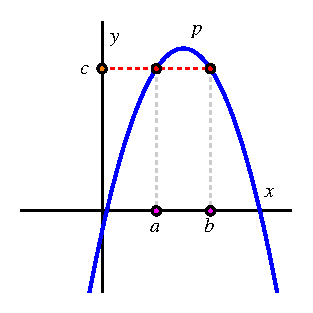
\includegraphics{inverse-does-it-1.pdf}
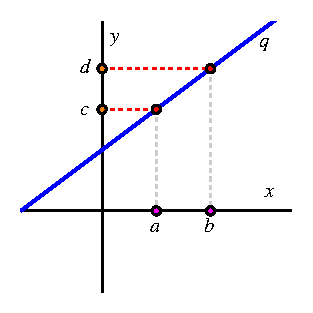
\includegraphics{inverse-does-it-2.pdf}
\end{image}

Recall that when a point such as $(a,c)$ lies on the graph of a function $p$, this means that the input $x = a$, which represents to a value on the horizontal axis, corresponds with the output $y = c$ that is represented by a value on the vertical axis.  In this situation, we write $p(a) = c$.  We note explicitly that $p$ is a function because its graph passes the vertical line test: any vertical line intersects the graph of $p$ exactly, and thus each input corresponds to one and only one output.

If we attempt to change perspective and use the graph of $p$ to view $x$ as a function of $y$, we see that this fails because the output value $c$ is associated with two different inputs, $a$ and $b$.  Said differently, because the horizontal line $y = c$ intersects the graph of $p$ at both $(a,c)$ and $(b,c)$ (as shown in the figure), we cannot view $y$ as the input to a function process that produces the corresonding $x$-value.  Therefore, $p$ does not have an inverse function.

On the other hand, provided that the behavior seen in the figure continues, the function $q$ does have an inverse because we can view $x$ as a function of $y$ via the graph.  This is because for any choice of $y$, there corresponds one and only one $x$ that results from $y$.  We can think of this visually by starting at a value such as $y = c$ on the $y$-axis, moving horizontally to where the line intersects the graph of $p$, and then moving down to the corresonding location (here $x = a$) on the horizontal axis.  From the behavior of the graph of $q$ (a straight line that is always increasing), we see that this correspondence will hold for any choice of $y$, and thus indeed $x$ is a function of $y$.  From this, we can say that $q$ indeed has an inverse function.  We thus can write that $q^{-1}(c) = a$, which is a different way to express the equivalent fact that $q(a) = c$.

The two examples above illustrate an important requirement for a function to have an inverse function. For a function to have an inverse, different inputs must go to different outputs, or else we will run into the same problems as we did in the examples of $f$ and $p$ above.

\begin{definition}
A function $f$ is said to be  \index{function ! one-to-one}\index{one-to-one function}\index{one-to-one}\dfn{one-to-one} if $f$ matches different inputs to different
outputs. Equivalently, $f$ is one-to-one if and only if whenever $f(a) = f(b)$, then $a = b$. If a function is one-to-one, it has an inverse.
\end{definition}

In particular, the graphical observations that we made for the function $q$ in the last example provide a general test for whether or not a function given by a graph has a corresponding inverse function. 

\begin{remark}
A function whose graph lies in the $x$-$y$ plane is one-to-one if and only if every horizontal line intersects the graph at most once.  When the graph passes this test, the horizontal coordinate of each point on the graph can be viewed as a function of the vertical coordinate of the point. This is sometimes referred to as \index{horizontal line test}\emph{the horizontal line test}.
\end{remark}



\begin{exploration}
Consider the functions $r$ and $s$ defined by
$$
y = r(t) = 3 - \frac{1}{5}(t-1)^3 \text{ and } y = s(t) = 3 - \frac{1}{5}(t-1)^2.
$$


\begin{enumerate}[label=\alph*.]
\item Solve the equation $y = r(t)$ for $t$. Can $t$ be expressed as a single function of $y$? What could go wrong?
\item Is $r$ one-to-one?
\item Find $s(2)$ and $s(0)$. Compare them; is $s$ is one-to-one?
\item Solve the equation $y = s(t)$ for $t$. Can $t$ be expressed as a single function of $y$? What could go wrong?
\end{enumerate}
\end{exploration}

To check your answers for b. and c. above, you could try graphing $r$ and $s$ and applying the horizontal line test. 

%\typeout{************************************************}
%\typeout{Graphical properties of inverse functions}
%\typeout{************************************************}

\section{Graphical properties of inverse functions}
Finally, we mention an important relationship between the graph of a function and the graph of its inverse function. If $f$ is one-to-one, then recall that a point $(x, y)$ lies on the graph of $f$ if and only if $y = f(x)$. From this, since $f$ is one-to-one, we can equivalently say that $x = f^{-1}(y)$.  Hence, the point $(y,x)$ lies on the graph of $x = f^{-1}(y)$.

The last item above leads to a special relationship between the graphs of $f$ and $f^{-1}$ when viewed on the same coordinate axes.  In that setting, we need to view $x$ as the input of each function (since it's the horizontal coordinate) and $y$ as the output.  If we know a particular input-output relationship for $f$, say $f(-1) = \frac{1}{2}$, then it follows that $f^{-1} \left( \frac{1}{2} \right) = -1$.  We observe that the points $\left(-1, \frac{1}{2} \right)$ and $\left(\frac{1}{2}, -1 \right)$ are reflections of each other across the line $y = x$.  Because such a relationship holds for every point $(x,y)$ on the graph of $f$, this means that the graphs of $f$ and $f^{-1}$ are reflections of one another across the line $y = x$, as seen in the figure below.

\begin{image}
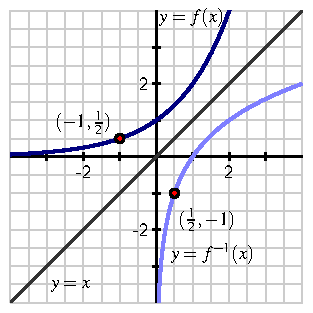
\includegraphics{inverse-plot-reflection.pdf}
\end{image}

\begin{summary}\begin{itemize}
\item We say a function $f$ has an inverse function $g$ if $g(f(a)) = a$ and $f(g(b)) = b$ for all $a$ and $b$. We often use the notation $f^{-1}$ for $g$.
\item We say a function is one-to-one if it matches different inputs to different outputs. We can check graphically if a function is one-to-one with the horizontal line test. All one-to-one functions have inverses, and vice versa. 
\item The graph of $f^{-1}$ is the graph of $f$ reflected across the line $y = x$.
\end{itemize}\end{summary}

\end{document}
